\documentclass[onecolumn, draftclsnofoot,10pt, compsoc]{IEEEtran}

\usepackage{graphicx}
\usepackage{url}
\usepackage{setspace}
\usepackage{geometry}
\usepackage{listings}

\geometry{textheight=9.5in, textwidth=7in}

% 1. Fill in these details
\def \CapstoneTeamName{			              			 PlanteR-GB}
\def \CapstoneTeamNumber{					           			 Group 64}
\def \GroupMemberOne{				           				Austin Hodgin}
\def \GroupMemberTwo{				           				Travis Hodgin}
\def \GroupMemberThree{			            Maximillian Schmidt}
\def\GroupMemberFour{		        	               Zach Lerew}
\def \CapstoneProjectName{	      	    Winter is Coming...}
\def \CapstoneSponsorCompany{		    Oregon State University}
\def \CapstoneSponsorPerson{		 			  				 Victor Hsu}

% 2. Uncomment the appropriate line below so that the document type works
\def \DocType{		%Problem Statement
				Requirements Document
				%Technology Review
				%Design Document
				%Progress Report
				}

\newcommand{\NameSigPair}[1]{\par
\makebox[2.75in][r]{#1} \hfil 	\makebox[3.25in]{\makebox[2.25in]{\hrulefill} \hfill		\makebox[.75in]{\hrulefill}}
\par\vspace{-12pt} \textit{\tiny\noindent
\makebox[2.75in]{} \hfil		\makebox[3.25in]{\makebox[2.25in][r]{Signature} \hfill	\makebox[.75in][r]{Date}}}}
% 3. If the document is not to be signed, uncomment the RENEWcommand below
\renewcommand{\NameSigPair}[1]{#1}

%%%%%%%%%%%%%%%%%%%%%%%%%%%%%%%%%%%%%%%
\begin{document}
\begin{titlepage}
    \pagenumbering{gobble}
    \begin{singlespace}
    	%\includegraphics[height=4cm]{coe_v_spot1}
        \hfill

        % 4. If you have a logo, use this includegraphics command to put it on the coversheet.
        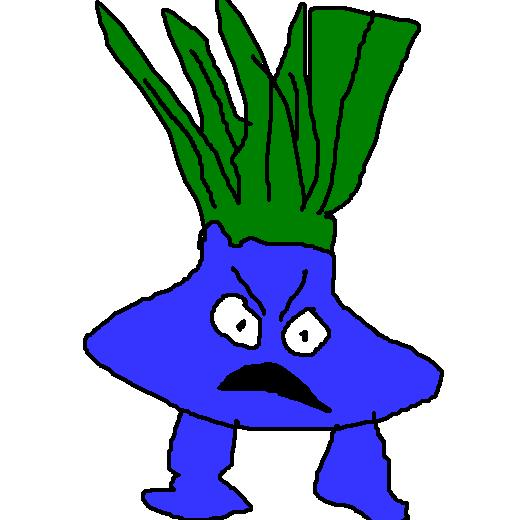
\includegraphics[height=4cm]{derp.jpg}

        \par\vspace{.2in}
        \centering
        \scshape{
            \huge CS Capstone \DocType \par
            {\large\today}\par
            \vspace{.5in}
            \textbf{\Huge\CapstoneProjectName}\par

            %\vfill
						\vspace{1in}

            {\large Prepared for}\par
            \Huge \CapstoneSponsorCompany\par
            \vspace{5pt}
            {\Large\NameSigPair{\CapstoneSponsorPerson}\par}

						\vspace{1in}

            {\large Prepared by}\par
						{\huge \CapstoneTeamNumber}\par
            \CapstoneTeamName\par
            \vspace{5pt}

            {
							\Large
							\NameSigPair{\GroupMemberOne}\par
							\NameSigPair{\GroupMemberTwo}\par
							\NameSigPair{\GroupMemberThree}\par
							\NameSigPair{\GroupMemberFour}\par
            }

            \vspace{20pt}
        }

				\newpage
        \begin{abstract}
				\noindent This project will create a system that controls RGB LEDs responsible for indoor plant growth during the cold seasons.
				Seasonal weather conditions may vary between different parts of the world, but plant growth becomes especially difficult during the fall and winter months.
				Oregon is an exceptional case of this rule. The state's winter season produces a hostile growth environment for plants such as herbs, spices, and decorative flowers.
				Plants like these are not able to survive the cold, dark, and humid Oregon weather.

				\noindent Bringing the plants into a more friendly and manageable indoor environment can still prove to be a difficult task.
				Plants need specific conditions for soil, water, temperature, and light.
				Existing indoor lighting systems can be difficult to use, expensive, and provide few customization options.
				Research provided by the client \textbf{\textsuperscript{citation needed}} has shown that some plants grow differently under different colors(wavelengths) of light.
				This project aims to produce a system that can control the color, intensity, and schedule for multiple zones of RGB LEDs.
				The system produced by these efforts will have a simple user interface through which all control settings can be viewed and manipulated.

				\noindent Once given control over the growing conditions, the plants will have a better chance of successful growth, and at the same time the impact on the user's busy life will be reduced.
				The system will be driven by a microprocessor that will manipulate the color, intensity, and schedule for multiple zones of RGB LEDs.
				Along side this hardware, the development of an intuitive user interface will allow the user to control the system with minimal physical interaction.
				The project has a simple core, but many stretch goals have been designed to increase functionality and end usability should time allow.

        \end{abstract}
    \end{singlespace}
\end{titlepage}

\newpage

\pagenumbering{arabic}
\tableofcontents
% 7. uncomment this (if applicable). Consider adding a page break.
%\listoffigures
%\listoftables
\clearpage
\singlespace


	% Document body
	\section*{Introduction}

		\subsection*{Purpose}

		\subsection*{Scope}

		\subsection*{Definitions, Acronyms, and Abbreviations}

		% References
		\subsection*{References}
		%\cite[Sec 3.8]{sourceName}
		%\bibliographystyle{IEEEtran}
		%\bibliography{./ref}


		\subsection*{Overview}


	\section*{Overall Description}
		\subsection*{Product Perspective}

		\subsection*{Product Functions}

		\subsection*{User Characteristics}

		\subsection*{Constraints}

		\subsection*{Assumptions and Dependencies}

	\section*{Specific Requirements}

		\subsection*{Required features - v1.0}
		\begin{itemize}
			\item LED lighting for a single plant bed
			\begin{itemize}
				\item A simple LED strip with a single controller attached to a single planter
				\item Service running on a micro controller that can control the power state of attached LED lights
				\item Configuration settings for the light state is read from a configuration file
				\item Changes to the configuration file are recognized and applied by the controller
			\end{itemize}
			\item Color and intensity Control
				\begin{itemize}
					\item User can select the color and light intensity of the light strip
				\end{itemize}
			\item Lighting state schedule
				\begin{itemize}
					\item User can specify weekly and daily scheduling for the state of the light (Color, Intensity, Power)
				\end{itemize}
			\item Zoning for individual control over multiple strips
				\begin{itemize}
					\item Controller supports individual control of up to 20 zones
					\item Each zone can chain light strips together on one data pin
				\end{itemize}
			\item Simple user interface for basic control
				\begin{itemize}
					\item Simple interface to edit configuration settings and physically transfer changes to the controller
					\item All settings can be changed from this interface, though it may not be user friendly
					\item Controller recognizes configuration changes and applies them automatically
				\end{itemize}
		\end{itemize}

		\subsection*{Additional features - v2.0}
		\begin{itemize}
			\item Improved User Interface
			\begin{itemize}
				\item Hosted web interface on local network
				\item Easy to use and responsive interface that shows the current state of the system
				\item All system settings can be updated and applied over the network without the need for physical access to the controller
			\end{itemize}
			\item Sub zoning on an individual light strip
				\begin{itemize}
					\item Multiple colors and intensities on a single light strip using LED indexing
				\end{itemize}
			\item Flexible zoning and sub-zoning
				\begin{itemize}
					\item Whole light strips and sub strips can be zoned together for more precise lighting control
				\end{itemize}
			\item Mobile web interface
				\begin{itemize}
					\item Web interface adds mobile support
					\item Android application acting as a wrapper for the web interface
				\end{itemize}
			\item Custom enclosure with vertical lighting
				\begin{itemize}
					\item Custom designed planter that holds the controller and lights
				\end{itemize}
			\item Environmental monitoring
				\begin{itemize}
					\item Monitoring for humidity and temperature using additional hardware sensors
					\item Web interface plugin to monitor humidity and temperature
				\end{itemize}
		\end{itemize}

		\subsection*{Stretch goals - v3.0}
		\begin{itemize}
			\item Modular light strips and enclosure
				\begin{itemize}
					\item Easy to attach light strips are automatically detected and setup
					\item Snap together enclosures allow quick and effortless system control
				\end{itemize}
			\item Gardening guide built into interface to help user learn best gardening practices
				\begin{itemize}
					\item Interface provides tips and suggestions to improve growing and gardening
				\end{itemize}
			\item Modular planting enclosure with snap together components
				\begin{itemize}
					\item Self contained enclosures with plug-and-play connectors for automatic and hassle free setup of multiple planters
				\end{itemize}
			\item Irrigation system
				\begin{itemize}
					\item Hardware and software necessary to facilitate automatic or scheduled watering
					\item *Requires custom enclosure
				\end{itemize}
			\item Wireless control over multiple plant growth systems
				\begin{itemize}
					\item Ad hoc style wireless system to allow seamless control over multiple grow light systems
					\item Support for large distributed systems, such as greenhouses
				\end{itemize}
		\end{itemize}

	\section*{Performance Metrics}
	Defining performance metrics for this project has been a back and forth topic for this team. The client's requirements are easily met by a team of four people, but our internal expectations are much higher. To avoid feature bloat and to guarantee the product functions per the client's requirements at a minimum, the features below describe the features necessary to define the project as a success. Extra features will be added after the completion of these functionally required features.
	\begin{itemize}
		\item \textbf{All features described by the client} listed in section \textit{Required features} are complete.
		\item An alternative interface as described in \textit{Additional features}. An interface that allows all controller settings to be modified without \textit{physical access to the controller}.
		\begin{itemize}
			\item This interface will likely be a web server hosted on the controller, but is subject to change as the project evolves.
		\end{itemize}
	\end{itemize}


\end{document}
